\chapter{GUI application}
\label{chap:GUIApplication}

The GUI application is based on \myProperNameImp{XULRunner}\footnote{\url{https://developer.mozilla.org/en/XULRunner}}, an application framework developed by \myProperName{Mozilla} and as such also known as the Mozilla Framework. \myProperName{XULRunner} also serves as the foundation of popular applications like \myProperName{Mozilla Firefox}\footnote{\url{http://www.mozilla.org/en-US/firefox/}} and \myProperName{Thunderbird}\footnote{\url{http://www.mozilla.org/projects/thunderbird/}}. 

\myProperName{XULRunner} applications are mainly created using \myProperNameImp{XUL}\footnote{\url{https://developer.mozilla.org/en/XUL}} (XML User Interface Language - a markup-language similar to \myProperNameImp{HTML}\footnote{\url{http://www.w3.org/html/}}), \myProperNameImp{CSS}\footnote{\url{http://www.w3.org/Style/CSS/Overview.en.html}}(Cascading Style Sheets) and \myProperNameImp{JavaScript} (\myProperNameImp{ECMAScript}\footnote{\url{http://www.ecmascript.org/}}). \myProperName{XUL} can seamlessly be replaced with \myProperName{HTML} for markup, thus \myProperName{XULRunner} applications can be build using the same technologies as web pages. Unlike web pages though, \myProperName{XULRunner} is a full featured desktop application framework and as such provides functionality to access the operating system, for example for file manipulation. Most of this functionality can be accessed from \myProperName{JavaScript} using \myProperNameImp{XPCOM} (see \myRefSection{sec:ComponentModels}). \myProperName{XULRunner} can be extended with native code through \myProperName{XPCOM} binary components or access of shared libraries using \myProperNameImp{js-ctypes} (see \myRefSection{sec:DynamicFFI}).

The decision to create the GUI application using \myProperName{XULRunner} is mostly based on its easy extendability and customizability - both stated as design goals in \myRefChapter{chap:DesignGoals}. Similar to the \myProperName{Firefox} browser, users will be able to write extensions to provide support for new features, for example glue code generators for scripting languages not supported by the main application.\\
Being based on web technologies, especially \myProperName{JavaScript}, development with  \myProperName{XULRunner} is very fast.
\\Personal preference and experience with the framework have also been major factors.

\newpage
\section{Basic concept}
\label{sec:BasicConcept}

\begin{figure}[h] % h = here
	\centering
		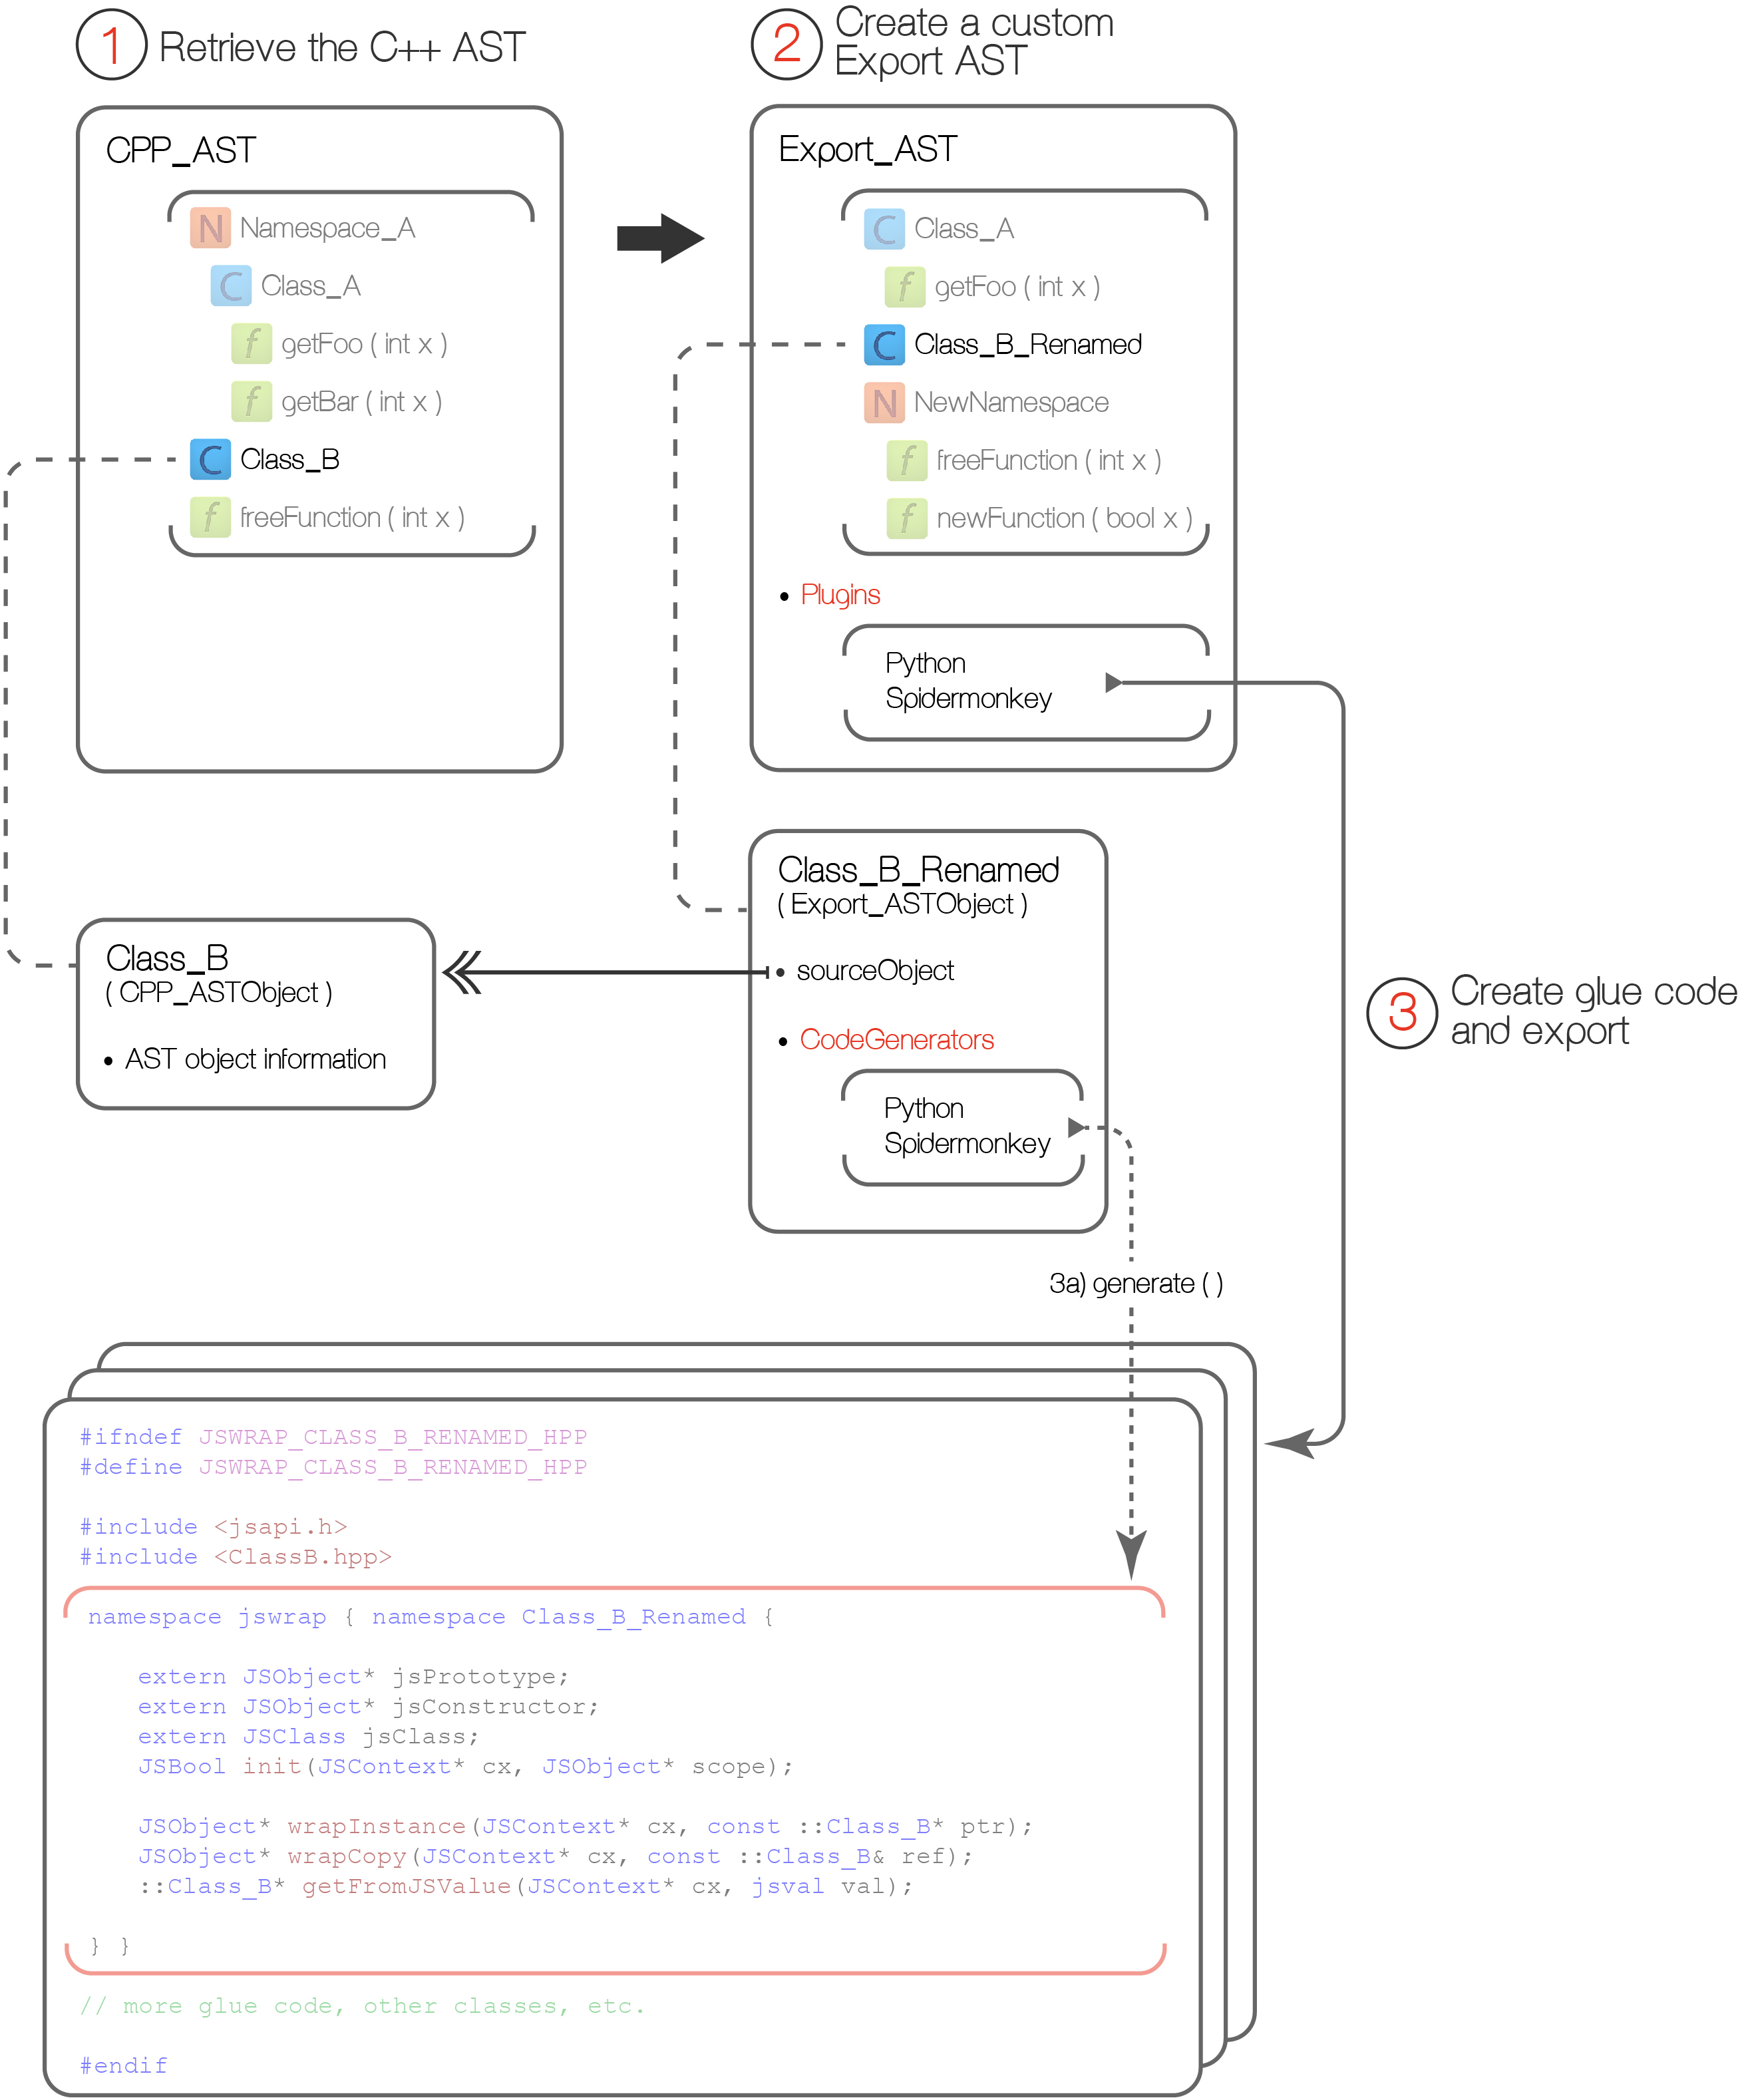
\includegraphics[scale=0.35]{Images/GUIApp_Concept.jpg}
	\caption{Basic concept}
	\label{fig:GUIAppConcept}
\end{figure}

In the first step, the application retrieves the \myProperName{C++} AST of a given source code file using \myProperName{CPPAnalyzer}. The data structures closely (but not completely) resemble the data structures used in \myProperName{CPPAnalyzer}. The information about the tree is hold in an instance of the \myProperName{JavaScript} class \mySCName{CPP\_AST} (equivalent to \mySCName{Clang\_AST}). This object holds a reference to the root tree node. All tree nodes are instances of subclasses of \mySCName{CPP\_ASTObject}.

Based on the elements in the \myProperName{C++} AST, the user will create a custom Export AST. This gives him the opportunity to alter the output of the application by choosing the AST nodes to be exported, rearranging the hierarchy and adding (artificial) nodes that are not in the original \myProperName{C++} AST. This gives the user complete control about how his C++ code can be accessed from script. Similar to \mySCName{CPP\_AST}, \mySCName{Export\_AST} holds a reference to the root tree node of the export tree. All tree nodes are instances of \mySCName{Export\_ASTObject}.

Both \mySCName{CPP\_AST} and \mySCName{Export\_AST} share the same base class \mySCName{AST}. \mySCName{ASTObject} is the base class of \mySCName{CPP\_ASTObject} and \mySCName{Export\_ASTObject}.

The glue code will be generated with the help of special code generator plugins/language plugins. The application can be extended to support glue code generation for arbitrary scripting languages. Based on the list of installed plugins, the user can add multiple plugins to the the existing \mySCName{Export\_AST}. In \myRefFigure{fig:GUIAppConcept} the plugins for \myProperName{Python} and \myProperName{Spidermonkey} have been added, while plugins for \myProperName{LUA} or \myProperName{PHP} may be installed, but are not needed for the user's project.

Every \mySCName{Export\_ASTObject} holds a list of code generators. Code generators are special classes provided by a plugin, which have the objective of generating the glue code for the specific \mySCName{Export\_ASTObject} they are connected to. The information used for the glue code generation is mostly retrieved from the \mySCName{Export\_ASTObject}s \mySCName{sourceObject}, which is usually a reference to a \mySCName{CPP\_ASTObject}. In \myRefFigure{fig:GUIAppConcept} \mySCName{Class\_B\_Renamed} uses the \myProperName{C++} class \mySCName{Class\_B} as its \mySCName{sourceObject}. Code generators also have a set of options that can be altered to influence the glue code generation.
Every plugin comes with a set of code generators that handle the different kinds of \mySCName{CPP\_ASTObject}s. Thus a plugin provides different code generators for handling functions, classes, and so on. 

When performing the final export of a plugin, it traverses all the \mySCName{Export\_ASTObject}s in the tree, uses the associated code generators to produce glue code pieces that are then combined and saved in files. These files can be included in \myProperName{C++} projects and used in conjunction with the embedded script interpreter to add script-support for the wrapped classes and functions.

\section{GUI overview}

workflow \todo{All that stuff}

\section{Architecture}

The application mainly contains three different types of files:

\begin{itemize}\addtolength{\itemsep}{-0.5\baselineskip}
\item \myProperName{XUL} files contain markup for the layout of the GUI
\item \myProperName{CSS} files provide design information for the GUI markup
\item \myProperName{JavaScript} files provide the programming logic for the GUI and the internal parts of the application
\end{itemize}

Most of the \myProperName{JavaScript} logic is placed in modules that are shared across multiple windows. As the \myProperName{JavaScript} language itself does not support module files (as, for example \myProperName{Python} does), \myProperName{Mozilla} integrated module support in \myProperName{XULRunner} with \myProperName{JavaScript code modules}\footnote{\url{https://developer.mozilla.org/en/JavaScript_code_modules/}}. These modules can be imported from any \myProperName{JavaScript} file using a special import command.

The \mySCName{Bound} module is the main module of the application and can be imported to have access to the whole application. It stores information about the current project and holds a reference to the main window in case access to the GUI elements is needed.

The \mySCName{CPPAnalyzer} module provides access to the \myProperName{CPPAnalyzer} library and as such is used for parsing \myProperName{C++} files and retrieving the AST information.

For easier maintenance, application logic and GUI logic is separated. All modules that provide logic for the user interface and specific GUI elements are in a subfolder called \mySCName{UI}. None of these modules is referenced from code outside of this folder, except by \myProperName{XUL} files and the \mySCName{Bound} module. This will make it easier to develop a command-line version of \myProperName{Bound} at some point in the future.

\subsection{Meta data}
\label{sec:MetaData}

A meta data system has been developed to equip \myProperName{JavaScript} objects (and ''classes'') with additional information that can be used for dynamic GUI element creation and serialization/deserialization.

It can be used after importing the \mySCName{MetaData} module.

\SingleSpacing
\begin{lstlisting}[language=JavaScript, caption=Adding meta data to \myProperName{JavaScript} objects]
Components.utils.import("chrome://bound/content/modules/MetaData.jsm")

function SomeClass()
{
	this._notImportant = "This member is neither viewable nor savable";
	this.editMe = "This member will be shown and editable in the GUI";
	this.saveMe = "This member will be saved upon serialization";
	this.showAndSaveMe = "This member is viewable (but readonly)
	                      and savable";
}

MetaData.initMetaDataOn(SomeClass.prototype)
   .addPropertyData("editMe",        { view: {}})
   .addPropertyData("saveMe",        { view: {}, load_save: {}})
   .addPropertyData("showAndSaveMe", { view: {readOnly: true}, 
                                       load_save: {}})
\end{lstlisting}
\OnehalfSpacing

The call to \mySCName{initMetaDataOn} will create a non-enumerable property called \mySCName{\_metaData} on the given object. \mySCName{addPropertyData} adds information about the property with the given name. What kind of data is provided depends on how the object shall be used in the future.
\\The \mySCName{ObjectExplorer} (see \myRefSection{sec:ObjectExplorer}), for example, will check every enumerable property to see if a) it contains meta data and b) if that meta data has the \mySCName{view} member. If so, the checked property (e.g. \mySCName{editMe}) will be visible, when the object is inspected and depending on the type of the property (which can also be forced in the \mySCName{view} object) a GUI element will be created dynamically.
\\The \mySCName{LoadSaveFromMetaData} module  (used in \myRefSection{sec:Project}), on the other hand, can be used to serialize and deserialize an object with \myProperName{JSON}. It checks the meta data for the existence of the \mySCName{load\_save} member. If it exists, the checked property (e.g. \mySCName{saveMe}) can be saved/loaded. The saving or loading process can be customized by providing \mySCName{save} and \mySCName{load} functions with the \mySCName{load\_save} object. If such functions are not provided, the property will be saved according to its type.

The meta data is usually not used in its raw state. As an instance of a class that inherits from another class can contain multiple meta data objects (for the base class, for the subclass and even for the instance itself), the meta data will usually be aggregated before using it. \mySCName{MetaDataAggregate} performs this task by traversing the prototype chain and collecting all existing meta data objects. If multiple meta data objects contain data about the same property, the data of the subclass shadows the data of the base class for that property.

The meta data system is a core component of the application and plays a grand role in the maintainability of the source code as well as the customizability of the generated output and the application itself.

\section{The \myProperName{C++} AST}
\label{sec:CPPAST}

The \myProperName{C++} is retrieved by calling the \mySCName{parse\_header} function of the \myProperName{CPPAnalyzer} shared library (see \myRefSection{sec:CallingCPPAnalyzer}).

As \myProperName{CPPAnalyzer} exposes a \myProperName{C} interface, it can be used from \myProperName{JavaScript} with the help of \myProperName{js-ctypes}. As explained in \myRefSection{sec:DynamicFFI}, glue code needed to be written in \myProperName{JavaScript} to wrap the functionality of the library. The \mySCName{CPPAnalyzer} module contains the according code and can be imported to use the \myProperName{CPPAnalyzer} library.

\mySCName{parse\_header} returns the stringified JSON representation of the \myProperName{C++} AST, as shown in \myRefSection{sec:ExportJSON}. The string is deserialized into a \myProperName{JavaScript} object using \myProperName{JavaScript}'s \mySCName{JSON.parse} function.

In the next step an instance of \mySCName{CPP\_AST} including the AST nodes (\mySCName{CPP\_ASTobject}s) needs to be created from the result object. The AST nodes from \myProperName{CPPAnalyzer} shown in \myRefFigure{fig:ASTObjectUML}: \textbf{\mySCName{ASTObject} classes and \mySCName{ASTType}} have equivalents in \myProperName{JavaScript}, which mostly have the same properties. The \myProperName{JavaScript} class \mySCName{CPP\_ASTObject\_Namespace}, for example, is the equivalent to the \myProperName{C++} class \mySCName{ASTObject\_Namespace}.\\
The result object is traversed and \mySCName{CPP\_ASTObject}s and \mySCName{CPP\_ASTType}s created from the according objects. As the AST nodes and types cross-reference each other, this happens in two steps. This is necessary, because an object referenced may not have been created yet in case it is defined later in the tree.\\
First, instances of the according classes are created, but only with information about the name, id and parent of the AST object. Thus the final tree is already formed, though lacking specific information about its members. Types are created in a similar way. For both, the newly created objects are kept track of with a map that associates ids and AST nodes.\\
In the second step, the created objects are updated and missing information for all nodes and types is retrieved. If a cross-reference is found, the according AST node or type is looked up using the id-maps.

\section{The Export AST}

\section{Code generation}

This section will explain the basic concept behind code generation plugins, especially for language bindings. Adding code generation support for a scripting language is exemplified with the code generation plugin written for \myProperName{Mozilla Spidermonkey}.

As explained in \myRefSection{sec:BasicConcept}, the code generation is not based on the \myProperName{C++} AST itself, but on an export AST, whose \mySCName{Export\_ASTObject}s reference the \mySCName{CPP\_ASTObject}s as their \mySCName{sourceObject}. The export AST only includes the nodes the user wants to export. The nodes can be rearranged, renamed and \mySlang{artificial} nodes can be added. 

To create glue code for a specific scripting language, the user needs to add an instance of the according language plugin to the export AST. The language plugin only controls the code generation and exports the final files. The creation of the glue code itself happens with the help of the entity code generators. If the user wants to export a specific \myProperName{C++} entity to \myProperName{Spidermonkey}, for example the function \mySCName{foo}, an instance of the \myProperName{Spidermonkey} function code generator needs to be added to the according \mySCName{Export\_ASTObject}. The entity code generators come with the according language plugin. All in all this means that the user can create \textbf{one} export AST for exporting glue code for \textbf{multiple} languages. If an \mySCName{Export\_ASTObject} does not have an entity code generator for a specific target language, this object is simply not exported for that language.

Every language plugin inherits from the class \mySCName{LanguageBindingCodeGenPlugin}, which itself inherits from \mySCName{BaseCodeGenPlugin}. As the name suggests \mySCName{BaseCodeGenPlugin} defines the basic functionality for all kinds of code generation plugins (e.g. type library or documentation generators), whereas \mySCName{LanguageBindingCodeGenPlugin} adds functionality related to language binding. The entity code generators themselves have a similar hierarchy, inheriting from \mySCName{LanguageBindingEntityCodeGen}, which inherits from \mySCName{BaseEntityCodeGen}.

\mySCName{BaseCodeGenPlugin} provides dummy implementations for loading and saving the plugin. Every plugin also has to provide a property named \mySCName{context}, which declares the purpose of the plugin. The \mySCName{context} of the \myProperName{Spidermonkey} plugin is \mySCString{CPP\_Spidermonkey}, as it binds C++ and Spidermonkey. The \mySCName{context} is the entry under which plugins are stored in the \mySCName{Export\_AST} (and entity code generators in the \mySCName{Export\_ASTObject}).
\\Every instance of \mySCName{BaseEntityCodeGen} and its subclasses stores a reference to the plugin it was created from and to the \mySCName{Export\_ASTObject} for which it generates code. Besides dummy implementations for loading and saving, the \mySCName{BaseEntityCodeGen} also contains dummy implementations for \mySCName{prepareAndDiagnose} and \mySCName{generate}. These are the two main functions used in the generation process and will be explained in more detail later.

\subsection{Templates}

There are different ways of creating glue code for a target language. The generated glue code may make use of \myProperName{C++} features like namespaces, exceptions or templates. There a valid reasons, why an end-user might not want to or cannot use these features. If a scripting language provides a \myProperName{C}-API, it should be possible to create glue code in plain \myProperName{C}. Either way, the language plugin should not dictate the glue code style preferred by its developer.

For this reason, entity code generators make use of templates (not to confuse with \myProperName{C++} templates). A template is basically a string of \mySlang{incomplete} source code. It is \mySlang{incomplete} in the sense that it contains placeholders that will be filled with proper code when processing the template with the template engine. The template engine used in this project is \myProperName{jSmart}\todo{ref}, a \myProperName{JavaScript} port of the \myProperName{PHP} template engine \myProperName{Smarty}\todo{ref}.

\newpage
\SingleSpacing
\begin{lstlisting}[language=JavaScript, caption=Template for converting a \mySCName{bool} to \myProperName{JavaScript} in \myProperName{Spidermonkey}, label=lst:TemplateBool]
// declaring a template for converting a C++ bool to JS
var code = "jsval {$jsvalName} = BOOLEAN_TO_JSVAL({$inputVar});";

// creating the template
var template = new jSmart(code);

// processing the template
var result = template.fetch({jsvalName: "jsBool", 
                             inputVar:  "cppBool"});
                             
// result --> "jsval jsBool = BOOLEAN_TO_JSVAL(cppBool);"
\end{lstlisting}
\OnehalfSpacing

As can be seen in \myRefListing{lst:TemplateBool}, the template code contains the placeholders \mySCName{\{\$jsvalName\}} and \mySCName{\{\$inputVar\}}. After creating the \myProperName{jSmart} template by calling the \mySCName{jSmart} constructor, the \mySCName{fetch} function can be used to process the template. The function requires an argument that contains the values to be inserted for the placeholders (\mySCString{jsBool} and \mySCString{cppBool}).

Leaving the actual glue code generation to templates, the entity code generator's main task is to collect all the information needed, checking it for validity and passing it on to the template(s) for creating the final glue code. The code generator should thus be agnostic to different styles of glue code.

\subsubsection{Template manager and template files}

A \mySCName{TemplateManager} has been developed to manage and load templates from\linebreak files based on string identifiers. Using the \mySCName{getTemplate} function passing \linebreak\mySCString{CPP\_Spidermonkey/function} will iterate over all search-paths looking for a file named \mySCName{function} inside a folder named \mySCName{CPP\_Spidermonkey} (using \mySCName{.jsmart} or \mySCName{.js} as the file extension). If such a file is found, it is loaded and a \mySCName{jSmart} template created from it and cached for the session. The second call to \mySCName{getTemplate} with the same identifier will return the cached template.\\
As the user can add new paths to the start of the search paths list (note: currently not exposed to the GUI), it is possible to shadow existing templates with custom versions.

In the first versions, template files were plain text files containing the code a \mySCName{jSmart} template will be based on. Additional needs arose. Templates were, for example, needed to be able to contain information about what \myProperName{C++} header files would need to be included if the template is used. To move more style out of the code generator into the templates, the templates started to need scripting capabilities. With these capabilities provided it seemed useful to have dependencies between templates so they can share code.\\
All of these features were added as needed. Instead of using plain text templates, the files needed to contain stringified \myProperName{JSON} that provides information about the template code, includes and functions. This approach lead to unexpected problems, as the \myProperName{JSON} specification does not allow whitespace or control characters (like new lines or tabs) for aligning properties. This made templates hard to read and maintain. Thus a preprocessing step had to be added that removed the whitespace between properties, but leaving whitespace inside strings intact. There were more drawbacks that needed to be worked around, like having to double-escape control characters in certain situations.
\\As the template file contained function source code in text-form, functions had to be dynamically created when loading a template with the help of \myProperName{JavaScript}'s \mySCName{Function} object constructor.

This system was completely rewritten to accommodate its drawbacks. Instead of having files that contain \myProperName{JSON} data, template files became normal \myProperName{JavaScript} files that are loaded at run-time using \myProperName{XULRunner}'s \mySCName{mozIJSSubScriptLoader} component. A template is not a \mySCName{jSmart} object anymore, but a simple \myProperName{JavaScript} object. This object serves as the global scope in which the script file is dynamically executed. Thus, all variables and functions declared in the script will be properties of the template object.\\
The script can declare a couple of special properties that are important for its behaviour. If a variable named \mySCName{templateCode} is declared, a \myProperName{jSmart} template will be created based on the content and added as the \mySCName{jSmartTemplate} property of the template object. Also, a \mySCName{fetch} function will be added that forwards the \mySCName{fetch} function of the \myProperName{jSmart} template. The functions \mySCName{onFetchBefore} and \mySCName{onFetchAfter} can be declared to manipulate the data passed to the \mySCName{fetch} function of the \myProperName{jSmart} template or to alter its result.

\SingleSpacing
\begin{lstlisting}[language=JavaScript, caption=Example of a template file, label=lst:TemplateBool]
// declaring the includes
var includes = ["#include <jsapi.hpp>"];

// declaring the template code
var templateCode = "\
	jsval {$jsvalName} = BOOLEAN_TO_JSVAL({$inputVar}); \
	 // {$randomComment}";

function onFetchBefore(fetchData)
{
	fetchData.randomComment = "Gimme " + Math.random() + "$";
}

function onFetchAfter(fetchData, fetchResult)
{
	return fetchResult + " please";
}
\end{lstlisting}
\OnehalfSpacing

When fetching the template with \mySCName{\{jsvalName: "jsBool", inputVar:  "cppBool"\}} the \mySCName{onFetchBefore} function will be called and add \mySCName{randomComment} to the data that will be passed to the \mySCName{jSmartTemplate}'s \mySCName{fetch} function. The final result may look something like this:

\SingleSpacing
\begin{lstlisting}[language=JavaScript, caption=Result of fetching a template]
jsval jsBool = BOOLEAN_TO_JSVAL(cppBool); // Gimme 0.342$ please
\end{lstlisting}
\OnehalfSpacing
\$\todo{remove}

When a code generator retrieves a template it can access all data declared in it. The \mySCName{includes} variable, for example, will be used to collect all necessary include files for the final export. There are also cases, where code generators call functions in templates to generate information that needs to be passed to other templates.

The new template approach only has one drawback: multiline strings used for big \myProperName{jSmart} templates have a cumbersome syntax in \myProperName{JavaScript}, as escaped new line characters (\textbackslash n) and backslashes need to be added inside the string. The current workaround is to provide an additional file with the same name but the \mySCName{.jsmart} extension, which contains the pure \myProperName{jSmart} code. The \myProperName{jSmart} template will use this file instead of the \mySCName{templateCode} variable then.

\subsubsection{Templates and customization}

Templates play a vital role in the ability to customize the application's output.

Using templates for glue code generation categorizes the developers/users into four groups: besides the \myProperName{Bound} main developers and language plugin developers, there can be language plugin template developers that create complete sets of templates (e.g. one set that creates glue code in plain \myProperName{C}, another that uses \myProperName{C++} features, etc.).  End-users can decide for a set by adding the set directory at the start of the search paths, so it will shadow the standard templates. The end-user can also decide to only shadow single templates for customizing the export of specific kinds of entities or edit a code generator (via GUI) to use a different template for its connected \mySCName{Export\_ASTObject} only\todo{ref}.

\subsection{Type resolution}

Glue code for converting between \myProperName{C++} and \myProperName{JavaScript} types is needed in several places, for example when converting the parameters and return values of wrapped functions.

Types can generally converted from \myProperName{C++} to the scripting language and verse visa.

There are templates for converting fundamental types like \mySCName{int}, \mySCName{bool} or \mySCName{float}, but it would be complicated to have a template for every single type, especially as all classes are wrapped in a similar way. That is the reason \textbf{type libraries} exist in \myProperName{Bound}. \textbf{Type library entries} are created by the class code generator and exist for every wrapped class. A type library entry contains information about the type, most importantly an identifier for it (the class' USR) and the include file needed when wrapping the type. Type library entries also provide restrictions, which define in which way a wrapped class can be used. Some types may not allow being passed as a parameter, others do not allow being created from a returned copy and similar. All type libraries use the same templates for conversion. The type library entry is passed to the templates, so they can create glue code for the specific type.\todo{all restrictions}\\
The plugin manages a type library -  a collection of all existing type library entries.

\mySCName{LanguageBindingEntityCodeGen} contains functions for retrieving the correct template for a given \mySCName{CPP\_ASTType}. The templates are retrieved using type maps and type library entries.\\
Type maps are simple maps that associate the string representation of a type (e.g. \mySCName{bool} or \mySCName{std::vector *}) with the string-id of a template. Every code generator contains two type maps, one for converting types from \myProperName{C++} to script and one for converting from script types to \myProperName{C++} types. All fundamental \myProperName{C++} types have type map entries stored in the type maps of the plugin, which serve as the \myProperName{JavaScript} prototypes of the type maps of the entity code generators. This is a natural way of shadowing. If a code generator's type map is asked for the template for \mySCString{bool}, but does not have such an entry, the type map of the plugin will be asked for \mySCString{bool} automatically as \myProperName{JavaScript} will traverse the prototype chain of the object. This concept is very handy for customization. If, for example, the user wants to change the template used for the \mySCName{bool} type for all occasions of the type, he will change the name of the template in the plugin's type map, as all code generators share the same plugin. If, on the other hand, he only wants to change how \mySCName{bool} is handled for one function, a type map entry for \mySCString{bool} in the type map of that specific code generator has to be added.

A single type can have multiple string representations, for example if typedef's are used. All of these string representations can be retrieved using the \mySCName{TypePrinter} class. The \mySCName{TypePrinter} can also be configured to create string representations with the \mySCName{const} classifier removed.

When trying to retrieve the template for handling a type, the application will try the following steps:

\begin{enumerate}
\item Based on the string representations of the type, the code generator's type map is checked for an according entry - starting with the most sugared version and ending with the canonical one. If an entry exists the according template is returned. If no type map entry exists, the type map will be checked for string representations of the same type with \mySCName{const} removed. Again, if an entry exists, the template is returned.
\item If the previous step didn't lead to any result and the type is a class or a pointer to a class, the plugin's type library is checked ther is an entry for the given class' USR. If so, the type library template will be returned together with the found type library entry.
\item If no type library entry was found, the steps 1 and 2 are repeated for all base classes of the given type. This makes sense, as a base class may have been wrapped and is the best substitute at this point (Note: step 3 is currently not implemented, but intended).
\item If the base classes didn't lead to any result and the type is a pointer or reference, the template for generic wrappers is used. Generic wrappers don't expose any functionality of the underlying type, but allow passing objects around between language borders. This is useful if an object does not need to be used from script, but is retrieved as the return of a \myProperName{C++} function and needs to be passed to another \myProperName{C++} function.
\item If none of he above steps worked, \mySCName{null} is returned indicating an error.
\end{enumerate}

This procedure should be illustrated with an example. The following function needs to be wrapped:

\SingleSpacing
\begin{lstlisting}[language=C++, caption=Example function illustrating type resolution]
int wrapMe(const WrappedClass& p1, OtherSubClass* p2);
\end{lstlisting}
\OnehalfSpacing

A type map entry exist for \mySCName{int}. A type library entry exists for \mySCName{WrappedClass}.

The according function code generator detects that it needs to handle two parameter types (script to \myProperName{C++}) and a return type (\myProperName{C++} to script).\\
For \mySCName{p1} the script-to-\myProperName{C++}-type map is checked for \mySCString{const ::WrappedClass \&}. As this does not yield a result, \mySCString{::WrappedClass \&} is checked next. No result either. As \mySCName{WrappedClass} is a \mySCName{class}, the type library is checked based on the USR. An entry exists and the template for converting a type with a type library entry from script to \myProperName{C++} is returned along with the found entry.\\
For \mySCName{p2} neither type map nor type library entry exist. The base classes of \mySCName{OtherSubClass} are checked, but don't find a template either. As \mySCName{p2} is a pointer, the template for retrieving a \myProperName{C++} object from a generic wrapper is returned.\\
For the return type of type \mySCName{int}, the type map for converting from \myProperName{C++} to script is checked for an entry. As an entry for \mySCString{int} exists, the according template will be returned.

\subsection{Preparation, diagnosis and generation}

User customized auto-generated source code is just as error-prone as human-written code, especially when working across programming language borders. Producing non-compilable code makes a language binding generator useless - producing code that has undefined behaviour, leads to crashes, memory leaks or data corruption on the other hand is even worse as it may keep the user in a false sense of safety\todo{word}. This is especially true when looking at the set of potential problems that \textbf{can} arise due to memory management issues shown in \myRefChapter{chap:LanguageBindingCPPJS}.\\
Thus, diagnosing potential error sources before generating glue code is an essential task of any language binding generator. Not everything can be checked though. If there is a typo in a used template, the error can only be found upon compilation.

As defined in \mySCName{BaseEntityCodeGen}, every entity code generator needs to provide two important functions: \mySCName{prepareAndDiagnose} (or more specifically \linebreak\mySCName{prepareAndDiagnoseRound}) and \mySCName{generate}.

The basic idea is that the generation process is split into multiple steps: first preparation and diagnosis, then generation as the second step.

\mySCName{prepareAndDiagnose} will accumulate all data that is necessary for the generation process. Most of the data will be retrieved from the \mySCName{Export\_ASTObject}, the \mySCName{sourceObject} and the options set for the entity code generator itself. All data is saved in a property named \mySCName{\_genInput}. While the data is accumulated, it is checked for various sources of errors. If errors or warnings occur, these are stored in \mySCName{\_genInput.diagnosis}.\\
The range of checks is broad.\\
The existence of templates that are referenced by the code generator (e.g. \mySCString{CPP\_Spider-monkey/function}) needs to be verified.\\
A function code generator that creates glue code for a member function needs to check if its \mySCName{Export\_ASTObject}'s parent is creating the glue code for the class that the member function belongs to. If not, the glue code will call the function on an instance of a totally different class, probably resulting in a run-time crash.\\
The name of the \mySCName{Export\_ASTObject}, which will serve as the name of the function in the target language, needs to be checked for signs that can not be used for identifiers in the scripting language.\\
Types need to be checked if they can be handled (by trying to retrieve the according type handling template). If a type from the type library is detected, it also needs to be verified that the type is used within the limitations/restrictions mandated by the type library. A specific class may, for example, not be allowed to use as a parameter due to memory ownership problems.\\
This is only a short list. There are many more possible checks, which mostly depend on the nature of the code generator and target language. 

When creating such a system, it is important to be able to alter the diagnosis in certain situations, otherwise the diagnosis-system may perform its job to eagerly and limit the user. If the user is truly knowing what he is doing, he should be able to allow ignoring restrictions in certain situations. Especially type library restrictions are merely recommendations as they only point out \textbf{potential} risks. Options for ignoring certain diagnosis results have to be part of the code generator, but are currently not implemented.

Preparation happens in multiple rounds, meaning that the whole tree is traversed multiple times and \mySCName{prepareAndDiagnoseRound} called with the current round passed as an argument. This is necessary for cross-referencing. A function that needs a type library entry of a class that comes later in traversal would issue wrong errors, just because the according type library has not been created yet or is not up to date. Thus type library entries are created in the first round, while the functions just start preparing in the second round when it is safe to use the type library entries.

The final source code generation will only be executed, if there are no errors in the whole project. The \mySCName{generate} function of an entity code generator is used for producing the glue code for the according entity.  It only uses information stored in \mySCName{\_genInput} - identifiers, templates and other data needed for glue code generation. As explained in more detail in the following section, the \mySCName{generate} function will fetch the templates with the data provided. The method will return a \myProperName{JavaScript} object containing all information needed for assembling the export files, most importantly the glue code for the object. The result of a function code generator will, for example, contain the code for the wrapper function, as well as its name and all necessary include files. If the function belongs to a class, the class' code generator's \mySCName{generate} function will use this information for assembling the glue code of the whole class.

\subsection{The \myProperName{Spidermonkey} code generators}

To give a more practical example of the given information, the language plugin for \myProperName{Spidermonkey} and its code generators are explained in greater detail in this section.

The plugin, \mySCName{CPPSM\_Plugin}, contains two type maps for converting types between \myProperName{C++} and \myProperName{Spidermonkey}. These maps initially contain the templates for the conversion of fundamental types like \mySCName{int}, \mySCName{float} and \mySCName{bool}, but also for the conversion of strings (\mySCName{const char*} or \mySCName{std::string}) as string is a fundamental type in \myProperName{JavaScript}. The function \mySCName{getCodeGeneratorByASTObject} takes a \mySCName{CPP\_ASTObject} as an argument and returns the constructor for the appropriate entity code generator. For functions and member functions it returns the \mySCName{CPPSM\_FunctionCodeGen} constructor; for namespaces, classes and structs it returns the \mySCName{CPPSM\_ObjectCodeGen} constructor. Other \myProperName{C++} entities are currently not supported, but can easily be extended in a similar fashion.

\subsubsection{\mySCName{CPPSM\_FunctionCodeGen}}

As explained, \mySCName{CPPSM\_FunctionCodeGen} gathers all important information inside \mySCName{prepare}-\mySCName{AndDiagnoseRound}. As it uses type information, this is done in the second round. Nothing happens in the first.

The function first creates a new object for \mySCName{\_genInput} for a fresh start. It stores the name of the \mySCName{Export\_ASTObject}, as it will be used as the name of the \myProperName{JavaScript} function. Also the template that will be used for the function is retrieved by its name (standard is \mySCString{CPP\_Spidermonkey/function}). As all failed checks, an error message will be saved in the \mySCName{diagnosis} if the template cannot be found.\\
The method then checks if the according \mySCName{Export\_ASTObject} does have a \mySCName{sourceObject} and if that is a kind of function. For member functions, it will test if the parent \mySCName{Export\_ASTObject} wraps the according class. Information is stored about the function being declared as \mySCName{static} or if it is a call to an instance function. The name of the called \myProperName{C++} function and a string qualifying the scope of the function (f.ex. the class name) need to be stored as well. \\
Next, parameters will be added to the \mySCName{\_genInput}. For every parameter type the correct template information and type string are retrieved using \mySCName{getTypeHandlingTemplate} defined in \mySCName{LanguageBindingEntityCodeGen}. \mySCName{TYPE\_FROM\_SCRIPT} is passed for specifying the direction of type conversion. Templates are tested for existence. If the template information contains a type library entry, it will be tested if the type library entry allows the passing as a parameter (\mySCName{allowUnwrapping}).\\
The return type information is retrieved afterwards in a similar fashion, but with \mySCName{TYPE\_TO\_SCRIPT} as the direction. If the return type is a pointer or reference and a type library entry was found, it is checked if the wrapping of \myProperName{C++} instances is allowed (\mySCName{allowWrappingInstances}). If the type is a declaration, it is tested, if wrapping of copies is allowed (\mySCName{allowWrappingCopies}).\\
At the end, the necessary include file is retrieved based on the location information of the wrapped \mySCName{CPP\_ASTObject}. Without this file, the produced code could not be compilable as it would reference an undefined function.\\
If no errors were detected, the function returns \mySCName{true}.

For generation only information stored in \mySCName{\_genInput} is used. The \mySCName{generate} function returns an object containing all information needed for further assembling the generated glue code. This object contains a \mySCName{type} property, which is set to \mySCString{Function}. The object also stores information about the number of parameters, whether the function is static and the name under which the function should appear in script. Based on the parameter information in \mySCName{\_genInput}, the given templates for the parameters will be fetched to create the glue code for those. The same happens for the return type. In the next step, these glue code pieces and other information from \mySCName{\_genInput} are passed to the \mySCName{fetch} method of the template that creates the glue code of the whole function. The generated glue code, as well as the name of the wrapper function are stored in the result object.\\
All used templates (for parameters, return type and the function itself), will be checked if they provide include dependencies. All includes are collected, duplicates eliminated and the list stored in the result object, which is then returned.

\subsubsection{\mySCName{CPPSM\_ObjectCodeGen}}

\mySCName{CPPSM\_ObjectCodeGen} gathers all important information inside \linebreak\mySCName{prepareAndDiagnoseRound}. As it creates type library entries, this is done in the first round. Nothing happens in the second.

First the name for the class or scope is stored in \mySCName{\_genInput}. The names of all \linebreak\mySCName{Export\_ASTObject}s in the parent chain is retrieved as it can be used by the plugin. Also, depending on whether the \mySCName{exportObject} has children, the \mySCName{isInline} property will be set. Scopes or classes without children will not be saved in their own files.\\
\mySCName{CPPSM\_ObjectCodeGen} handles namespaces and \mySCName{Export\_ASTObject}s that do not have a \mySCName{sourceObject} different than classes. The glue code for the first group will only create a simple \myProperName{JavaScript} object and add functions to it. For classes, the glue code will create a complete \myProperName{JavaScript} class prototype and constructor function from which instances can be created. But as both groups share a lot of code, they are written in the same code generator.\\
For the first group, the \mySCName{type} property will be set to \mySCString{Object}. The templates for generating the header- and the source-file code will be retrieved. When not being adjusted by the user, these default to \mySCString{CPP\_Spidermonkey/hpp\_scope\_content\_object} and \mySCString{CPP\_Spidermonkey/cpp\_scope\_content\_object}.\\
For structs and classes the \mySCName{type} property will be set to \mySCString{Class} and the header and source-file templates will be retrieved defaulting to \mySCString{CPP\_Spidermonkey/hpp\_scope-\_content\_class} and \mySCString{CPP\_Spidermonkey/cpp\_scope\_content\_class}. Also, the full name including spaces is stored. A type library entry is created or updated and saved in the plugin based on the class' USR. The information for the type library is retrieved from the code generator and can be changed by the user from within the GUI. The type library entry is checked for incompatible options. For example, if the ownership is set to \mySCString{Native}, \mySCName{allowWrappingCopies} must be set to false, as wrapping copies returned from \myProperName{C++} functions would probably result in memory leaks, when memory is handled by the \myProperName{C++} side. The type library entry is also stored in \mySCName{\_genResult}, as is the include file in which the class was defined.\\
Again, if no errors occured, \mySCName{prepareAndDiagnoseRound} will return true.

The \mySCName{generate} function's first act is to call the \mySCName{generate} functions of all children resulting in a recursive generation. Thereby, the generation results of the children will be collected, as they will be passed to the templates. The templates are fetched. The templates for objects and classes internally iterate over the generation results of the children and if they find a result of \mySCName{type} \mySCString{Function}, the according glue code of the function will be inserted in the class' glue code.
The final step is to collect all used include files, just as \mySCName{CPPSM\_FunctionCodeGen} does.  The children results, the glue code  of the class (for header and source-files) and the \mySCName{isInline} property are stored in the result object and as such returned. \\

\subsubsection{Export}

The \mySCName{CPPSM\_Plugin}'s \mySCName{getExportFiles} function is responsible for assembling the code for the files to be saved upon export. It takes the generation result of a \linebreak\mySCName{CPPSM\_ObjectCodeGen} and tries to create complete files in a reasonable way. To do this, it traverses the generation results of the children recursively. If a child is marked \mySCName{inline}, then its content will be included in the same header and source file. Non-inline children will get their own set of files.\\
The content of the files will be assembled from the glue code and includes information found in the given generator result and its inline children generator results. The filenames of the created files are of course integrated into the include resolution process, as the glue code of scopes needs to call the \mySCName{init} functions of the child scopes so all elements will be correctly registered to the script interpreter.

The result of \mySCName{getExportFiles} is a map of filenames with their according source code.

\section{The project}
\label{sec:Project}

All project-related information is stored in a \mySCName{Project} object. The project basically stores a reference to the \mySCName{CPP\_AST} and the \mySCName{Export\_AST}. It also saves the options that were used for calling \myProperName{CPPAnalyzer}, in case the user needs to reparse the project with the same settings. The \mySCName{Project} class also contains functions for saving and loading a project.

\subsection{Saving}

A project is saved to two files: On the one hand there is the project file, which contains the \mySCName{Export\_AST} and other project settings in \myProperName{JSON}. The other file contains the \myProperName{JSON} of the \myProperName{C++} AST just as it was retrieved from \myProperName{CPPAnalyzer}.

For saving the \mySCName{Export\_AST}, its \mySCName{toSaveObject} function is called The function returns a JSON-compatible object, which can then be serialized for saving using \mySCName{JSON.stringify}. \mySCName{toSaveObject} does nothing, but calling the \mySCName{toSaveObject} functions of the root \linebreak\mySCName{Export\_ASTObject} (for saving all nodes) and the code generator plugins and stores the results in the \mySlang{save object} that it returns.\\
Upon saving, a \mySCName{Export\_ASTObject} needs to store the reference to its \mySCName{sourceObject} in a way that it can be retrieved again when loading. This is done by saving the \mySCName{CPP\_ASTObject}'s USR as an id. The export object also stores the save objects for all its children (thus saving recursively) and its own entity code generators associated with their \mySCName{context}. All of these different \myProperName{JavaScript} objects have their own \mySCName{toSaveObject} functions.

Most of the objects in the GUI application have meta data associated. As explained in \myRefSection{sec:MetaData}, this meta data can be used for saving and loading information. A simple implementation of a \mySCName{toSaveObject} function could look like this:

\SingleSpacing
\begin{lstlisting}[language=JavaScript, caption=Saving using meta data, label=lst:MetaDataSave]
function SomeClass()
{
	this.saveMe   = "Save me!";
	this.dontSave = "Don't dare saving me!";
}

// setting up the meta data
MetaData.initMetaDataOn(SomeClass.prototype)
   .addPropertyData("saveMe",  { load_save: {}})

// the toSaveObject function
SomeClass.prototype.toSaveObject = function toSaveObject()
{
	var result = {};
	
	// this call does all the magic
	LoadSaveFromMetaData.saveTo(result, this);
	
	return result;
}
\end{lstlisting}
\OnehalfSpacing

The result of calling \mySCName{toSaveObject} from \myRefListing{lst:MetaDataSave} would be the \myProperName{JavaScript} object \mySCName{\{ saveMe: "Save me!" \}}.

saving and loading, reparsing, metadata, etc., versioning

\subsection{Loading}

Loading is saving in reverse. The project file and the \myProperName{C++} AST file are loaded from disk. The \myProperName{C++} is created in the same way, as explained in \myRefSection{sec:CPPAST}. The contents of the project file are deserialized into a \myProperName{JavaScript} object using \mySCName{JSON.parse}. This is the exact \mySlang{save object} that was saved previously and as such can be loaded in a similar manner.\\
Some objects may have saved their type, so that the according instances can be created from the right class. Other objects may not have saved their type as it is retrieved by the given context. \mySCName{Export\_ASTObject}s need to set the correct \mySCName{CPP\_ASTObject} as their \mySCName{sourceObject}. This is done by querying the \mySCName{CPP\_AST} with the USR that was saved. If for whatever reason no \mySCName{CPP\_ASTObject} is found, the \mySCName{sourceObject} is set to \mySCName{null}, but the information about the correct object is stored for later in a property named \mySCName{\_sourceObjectSaveObject}. A warning may be issued in this case.\\
Loading from meta data works similarly to saving.\\
With the \mySCName{CPP\_AST} and the \mySCName{Export\_AST} instantiated, a new \mySCName{Project} instance is created for bundling the information again.

\subsection{Reparsing}

As the \myProperName{C++} projects for which glue code is created, may be under development, new functions or classes are likely to be added or removed. In such a case, the \myProperName{C++} AST has to be reparsed for the loaded project. A new \mySCName{CPP\_AST} is retrieved by calling \myProperName{CPPAnalyzer}. This invalidates all \mySCName{Export\_ASTObject}s as their \mySCName{sourceObject} properties still reference the old \mySCName{CPP\_ASTObject}s. Thus, the objects have to be reconnected to the new AST nodes by using the USRs of the old \mySCName{sourceObject}s. If the current \mySCName{sourceObject} is \mySCName{null}, the \mySCName{\_sourceObjectSaveObject} property is checked to recall information about the USR. If the \mySCName{sourceObject} is not \mySCName{null}, but the according USR is not in the new AST, then the old USR is stored in \mySCName{\_sourceObjectSaveObject} and the \mySCName{sourceObject} set to \mySCName{null}. This makes it possible to reconnect to the correct \mySCName{CPP\_ASTObject}, even if it got missing in a set reparse-operations, for example in case the \myProperName{C++} function/class/entity has been accidentally deleted in the source code and was readded later.

\section{GUI widgets}

\subsection{ObjectExplorer}
\label{sec:ObjectExplorer}

\subsection{DOMTree}

\begin{wrapfigure}{r}{0.4\textwidth}
  \begin{center}
    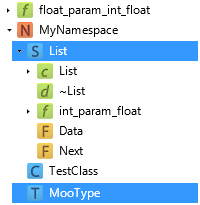
\includegraphics[scale=0.75]{Images/DOMTree.png}
  \end{center}
  \caption{Example of a \mySCName{DOMTree}}
  \label{fig:DOMTree}
   \vspace{-15pt}
\end{wrapfigure}

For displaying the \myProperName{C++} and export tree in the user interface a tree GUI widget has been written.

\myProperName{XUL} already comes with a native tree widget, but it requires the user to manage the hierarchy of visible tree elements in form of a list. The user himself has to track whether nodes have been opened and child nodes are visible and adjust the list accordingly.

As managing a tree structure in a list seemed rather complicated and styling a \myProperName{XUL} tree element works differently than styling any other \myProperName{XUL} or \myProperName{HTML} element (for performance reasons, it seems), I decided to create a new tree GUI widget, expressed in the class \mySCName{DOMTree}.

The widget makes use of the hierarchical nature of the \myProperName{XUL} \myProperName{Document Object Model (DOM)}. Tree elements are created dynamically at run-time using the \linebreak\mySCName{document.createElement} function. The tree basically consists of \myProperName{XUL} \mySCName{box} objects, which are \mySlang{instances} of \mySCName{DOMTreeRow}. As the \mySCName{box} box objects are created by the \myProperName{DOM}, they are not real instances of \mySCName{DOMTreeRow}, but borrow all its functions and properties. Borrowing functions allows using these as if they were declared in the object itself.\\
A \mySCName{DOMTreeRow} has a simple design. It is a vertical \mySCName{box} containing a title row (with twisty, symbol and label) and an initially empty vertical \mySCName{box} that serves as the child container. Child \mySCName{DOMTreeRow}s can be added to to the child container using the normal \myProperName{DOM} functions, e.g. \mySCName{element.appendChild}, resulting in a tree structure. The visual indentation is handled by \myProperName{CSS}.\\
When collapsing/opening a tree row by using the twisty, the container \mySCName{box}'s visibility is changed using the \myProperName{CSS} \mySCName{display} property - effectively hiding or showing all child rows.

Selection logic has been implemented for selecting individual or multiple tree rows. A \mySCName{selection} \mySCName{DOMEvent} is fired when the selection is changed.\\
Dragging of tree nodes has also been implemented based on the \myProperName{HTML5} drag-and-drop capabilities. \mySCName{DOMTreeRow} contains a private data field that will serve as the drag-data.

When creating a \mySCName{DOMTree} a callback function has to be passed. When creating a \mySCName{DOMTreeRow} this callback function is called to retrieve information about the GUI tree node, for example about the text label that should be used or styling attributes for setting the correct symbol.

\section{Known Problems}

from which file was a symbol included: need include file hierarchy


